\documentclass[aspectratio=169,11pt]{beamer}

\usetheme{Madrid}
\usecolortheme{default}
\usefonttheme{professionalfonts}
\setbeamertemplate{navigation symbols}{}
\setbeamertemplate{footline}[frame number]

\usepackage{amsmath, amssymb, booktabs, graphicx}
\graphicspath{{../../assets/figures/}{assets/figures/}}

\title{Wage Posting, Bargaining, and Wage-Setting}
\subtitle{Labor II --- Week 5}
\author{Teaching deck draft}
\date{}

\begin{document}

\begin{frame}
  \titlepage
\end{frame}

\begin{frame}{Central question and course repositioning}
\begin{itemize}
    \item Once workers and firms meet in a frictional labor market, how are wages actually set?
    \item Week 5 is the bridge from Week 4 search and job ladders to Week 6 monopsony and labor market power.
    \item The core distinction is between wage-setting protocols: posting, bargaining, and standardized or discretionary wage rules.
\end{itemize}
\end{frame}

\begin{frame}{Week 4 to Week 5 bridge}
\begin{itemize}
    \item Week 4 gave us meetings, vacancies, outside options, unemployment, and E-to-E mobility.
    \item Week 5 asks how those same objects shape wages inside the match.
    \item Search theory is incomplete until it specifies how surplus is converted into pay.
\end{itemize}
\end{frame}

\begin{frame}{Course map}
\begin{center}
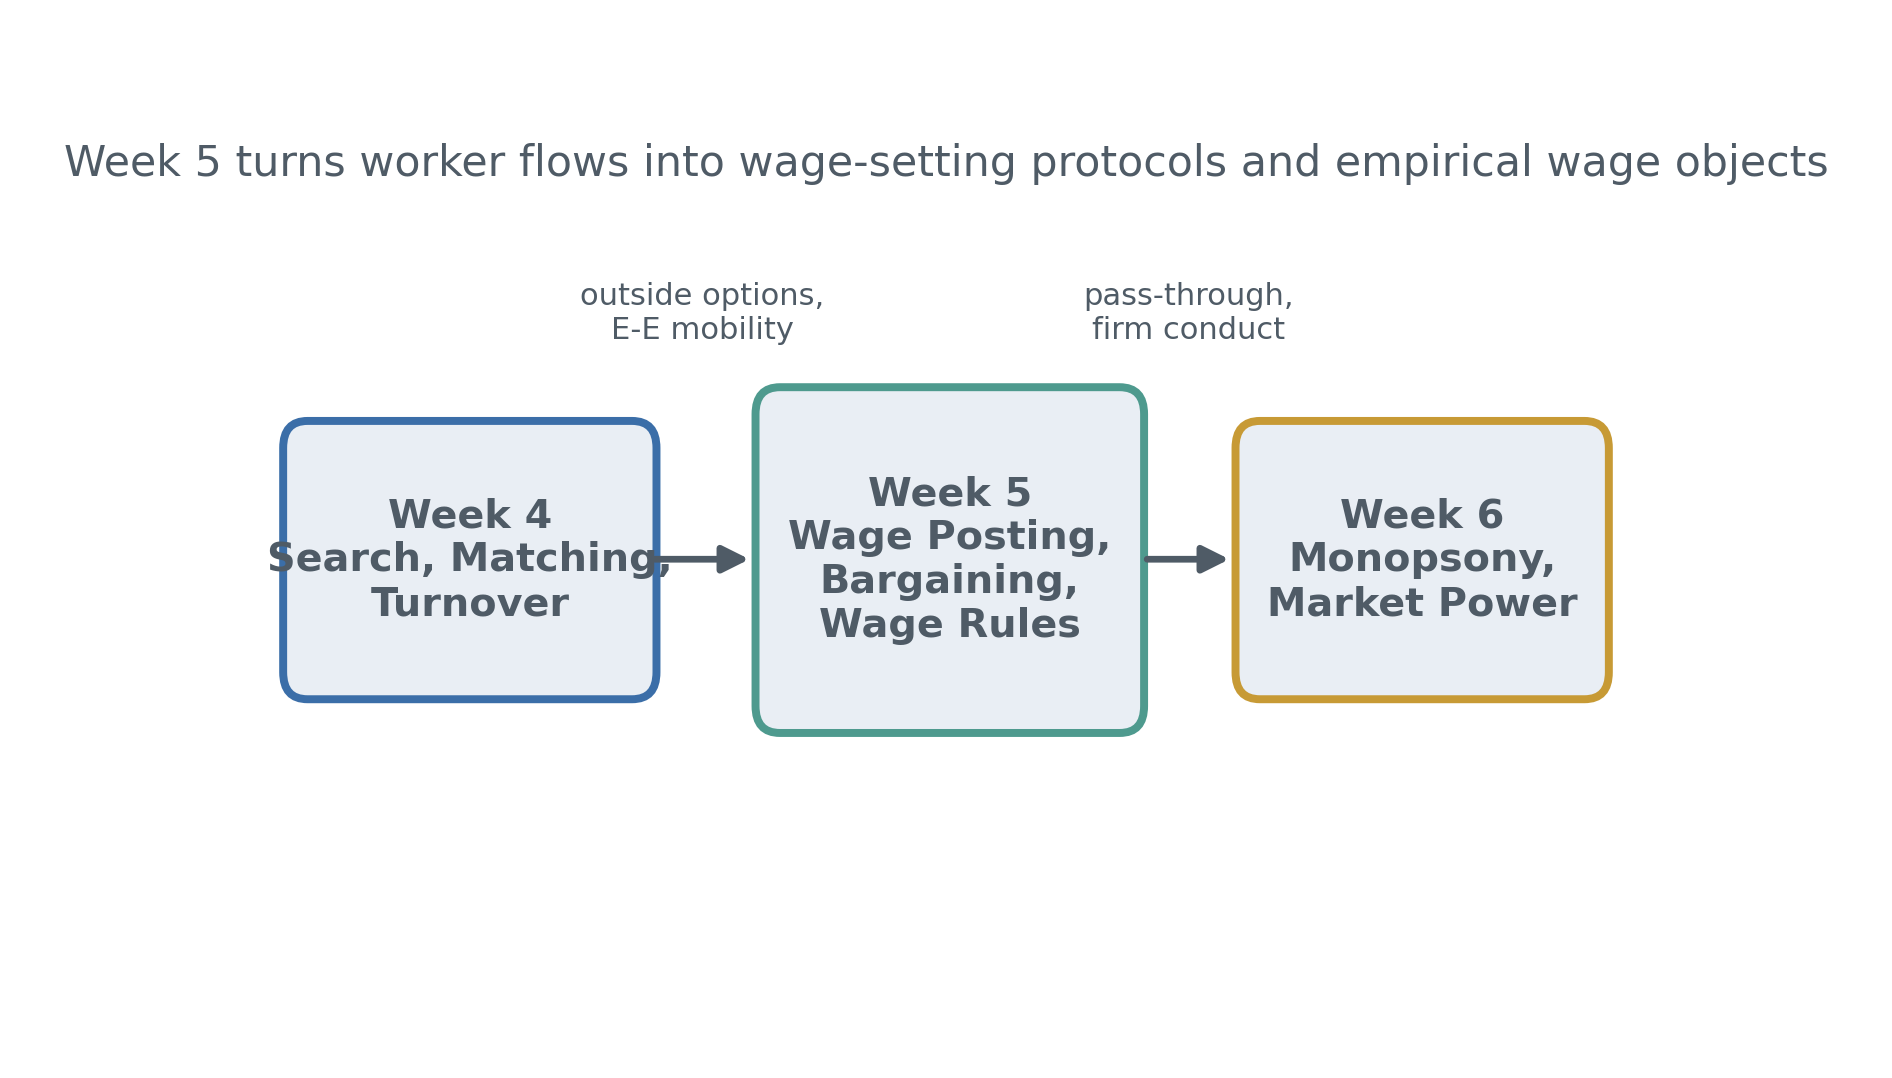
\includegraphics[width=0.9\linewidth]{05-wage-setting-course-map.png}
\end{center}
\end{frame}

\begin{frame}{Why search models need a wage-setting protocol}
\[
w \geq w^R
\quad \Leftrightarrow \quad
V^E(w) \geq V^U
\]

\begin{itemize}
    \item Acceptance is not yet a wage-setting protocol.
    \item The next question is whether the wage is posted, bargained, or constrained by a schedule.
    \item Frictions make labor supply to the firm finite rather than infinite.
\end{itemize}
\end{frame}

\begin{frame}{Competitive wages versus frictional wage setting}
\small
\begin{tabular}{p{0.23\linewidth} p{0.3\linewidth} p{0.38\linewidth}}
\toprule
Regime & Main wage object & Why wages differ \\
\midrule
Competitive benchmark & Market wage & Mostly worker or job productivity differences \\
Posted wage & Offer schedule chosen by firm & Recruiting and retention responses \\
Bargained wage & Negotiated wage & Surplus division, outside options, threat points \\
Standardized pay & Rule-based cell & Grades, steps, contracts, internal equity \\
Discretionary pay & Local managerial choice & Offer competition, retention, within-firm flexibility \\
\bottomrule
\end{tabular}
\end{frame}

\begin{frame}{Wage posting and the logic of wage dispersion}
\[
\max_w \; \pi(w) = (p-w)\,\ell(w)
\]

\begin{itemize}
    \item The firm chooses a wage anticipating how staffing responds.
    \item Burdett--Mortensen links employed search to wage dispersion and job ladders.
    \item The wage distribution is not automatically a productivity distribution.
\end{itemize}
\end{frame}

\begin{frame}{Posted wages versus individualized bargaining}
\begin{center}
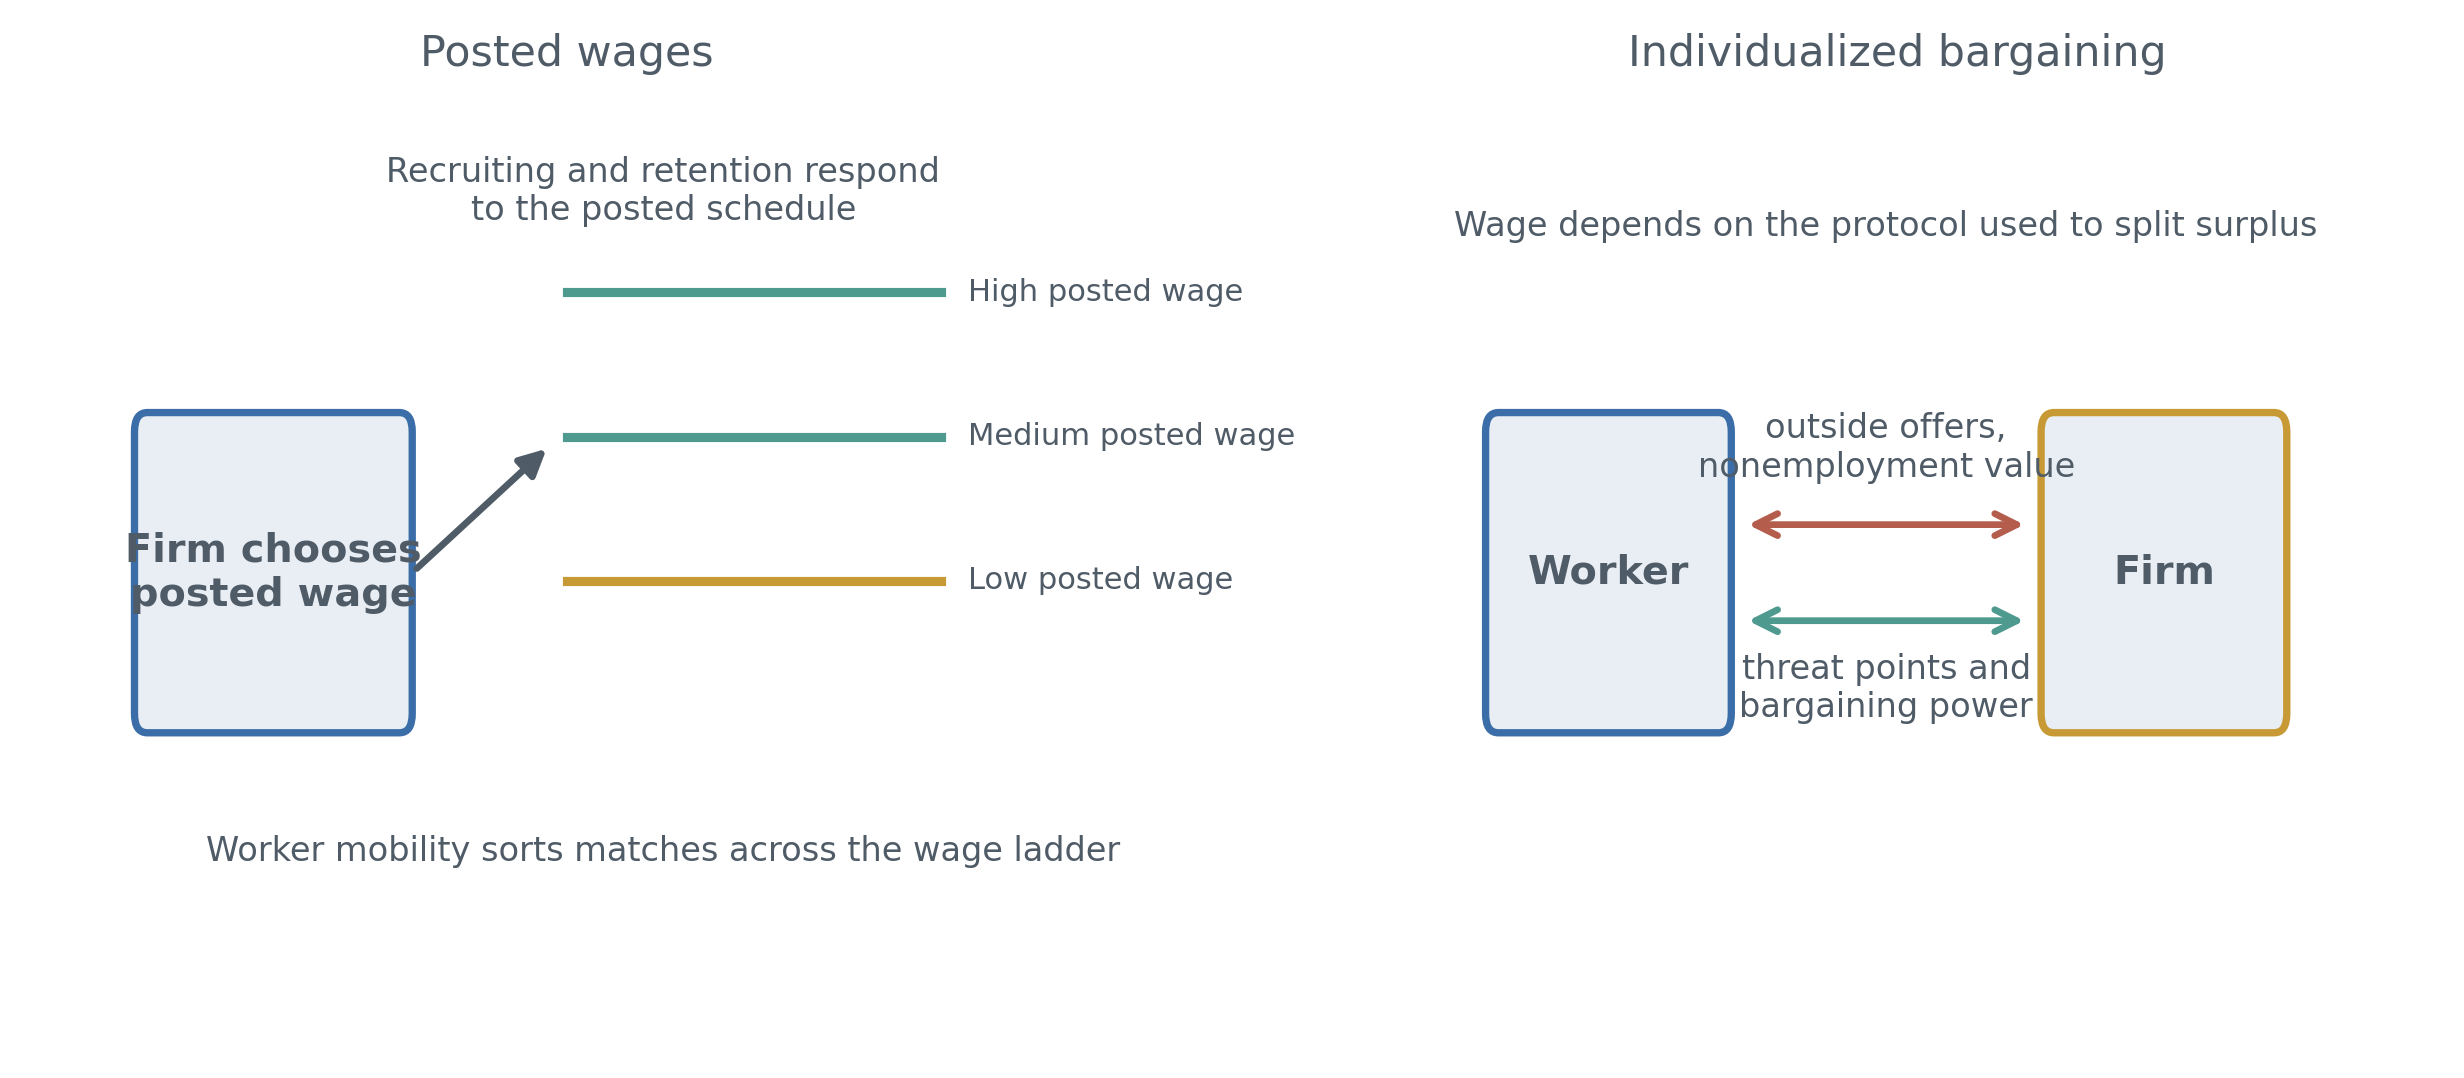
\includegraphics[height=0.72\textheight]{05-posting-vs-bargaining.png}
\end{center}
\end{frame}

\begin{frame}{Bargaining, outside options, and Hall--Milgrom}
\[
w^* = \arg\max_w \left[V^E(w)-V^U\right]^\beta \left[J(w)-V\right]^{1-\beta}
\]

\begin{itemize}
    \item Bargaining treats the wage as a bilateral surplus-splitting outcome.
    \item Outside options are not the same thing as threat points.
    \item Hall--Milgrom: if disagreement means delay rather than exit, unemployment may matter less for wages.
\end{itemize}
\end{frame}

\begin{frame}{Reservation wages, outside offers, threat points, and fallback values}
\begin{center}
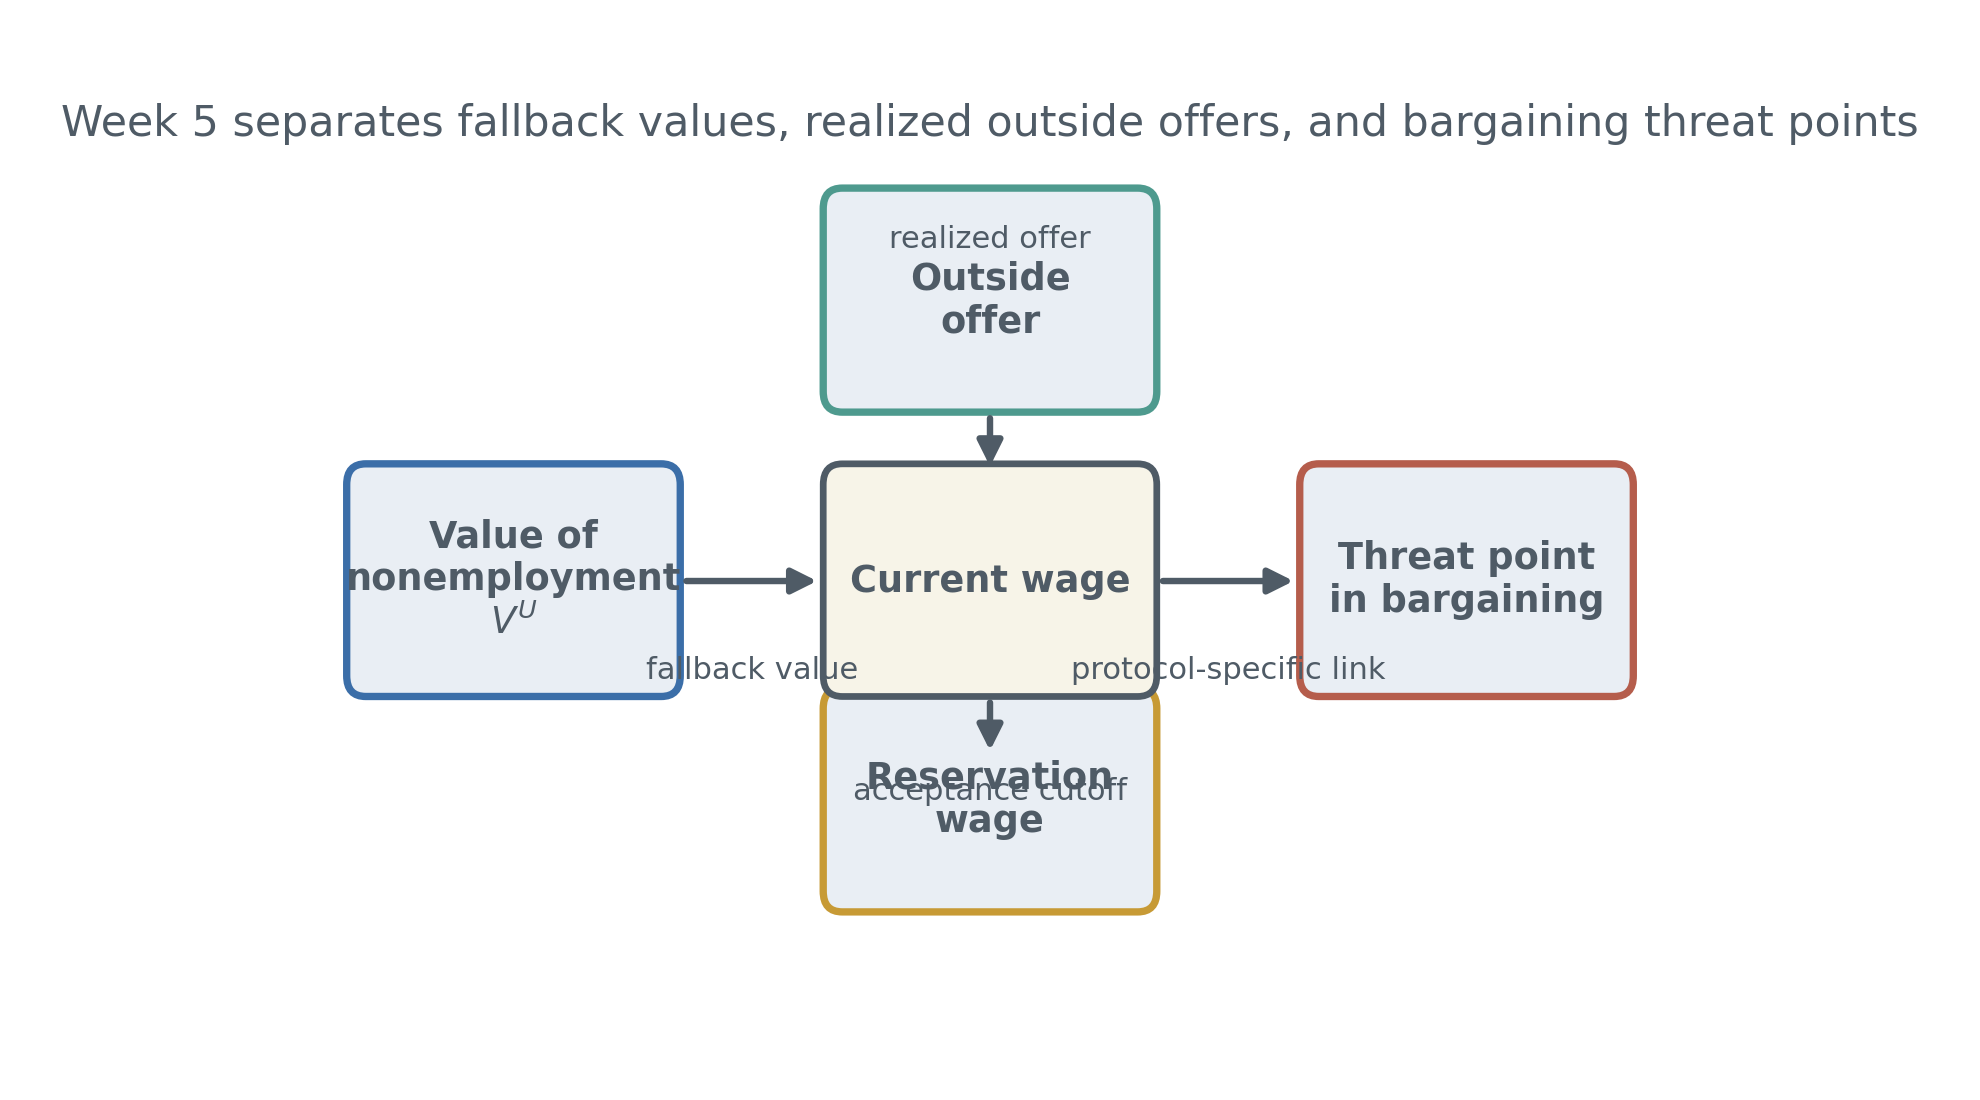
\includegraphics[height=0.72\textheight]{05-outside-options-and-wage-setting.png}
\end{center}
\end{frame}

\begin{frame}{Wages and the value of nonemployment}
\[
\Delta \log w_{it} = \rho \, \Delta \log V^U_{it} + \varepsilon_{it}
\]

\begin{itemize}
    \item A realized outside offer is not the same object as the value of nonemployment.
    \item Jaeger, Schoefer, Young, and Zweim\"uller ask how fallback values pass through to wages.
    \item This is distinct from pass-through from firm productivity or firm revenue shocks.
\end{itemize}
\end{frame}

\begin{frame}{Standardized versus discretionary pay-setting inside firms}
\begin{center}
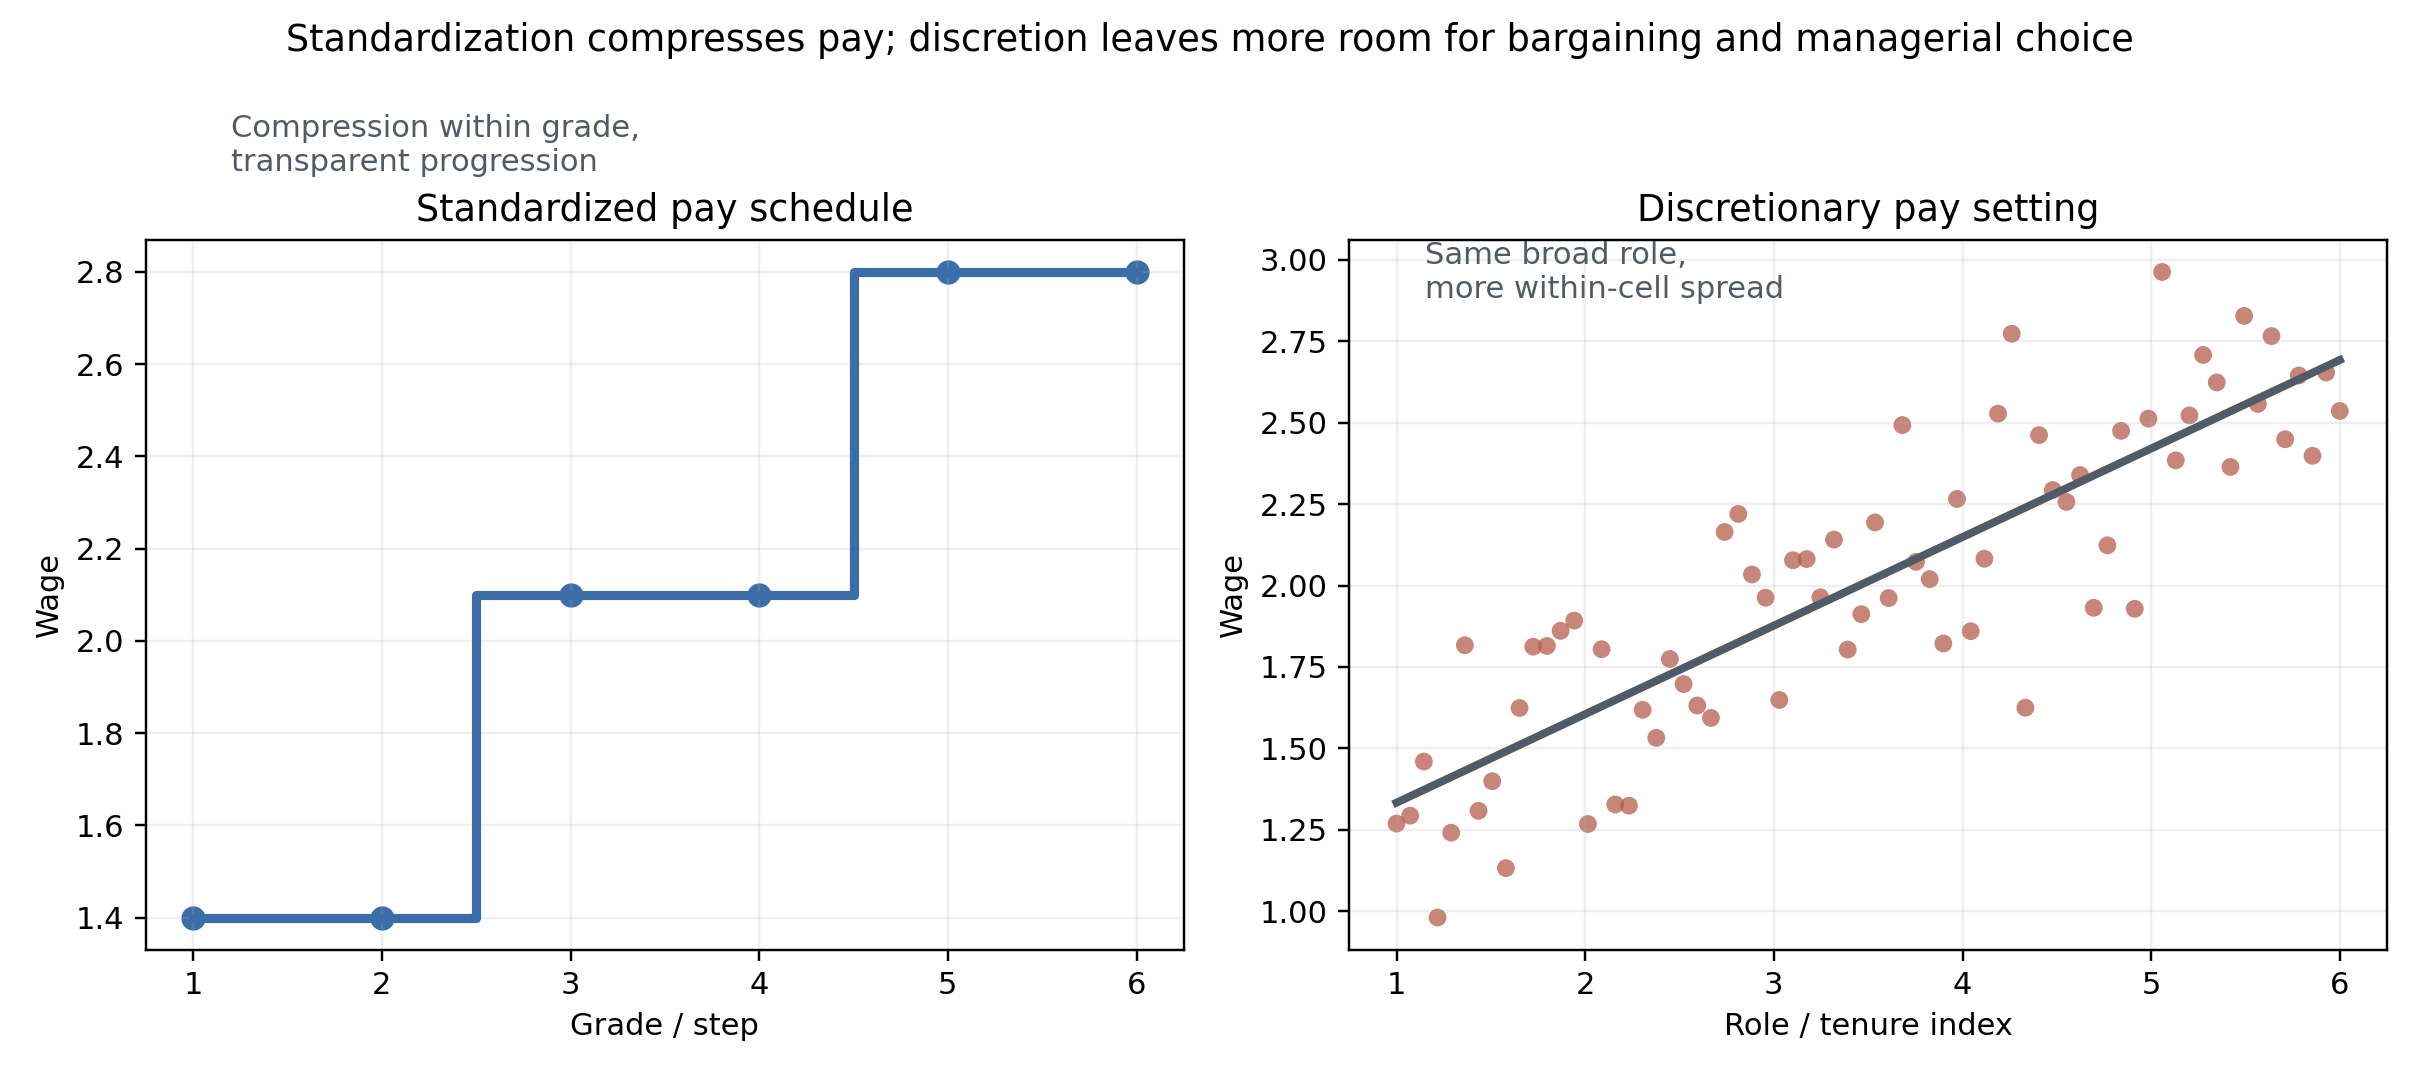
\includegraphics[height=0.72\textheight]{05-standardized-vs-discretionary-pay.png}
\end{center}
\end{frame}

\begin{frame}{Empirical designs and what they identify}
\small
\begin{tabular}{p{0.23\linewidth} p{0.2\linewidth} p{0.17\linewidth} p{0.27\linewidth}}
\toprule
Design & Variation & Margin & Main latent object \\
\midrule
Dual jobholders & Wage shock in other job & Wage vs separation response & Full offer set \\
Pay-rule reforms & Schedule or flexibility change & Compression, mobility, sorting & Nonwage job bundle \\
Nonemployment shocks & Fallback-value change & Wage pass-through & Expected search environment \\
Firm shocks & Value added or revenue change & Rent-sharing, premia & Sorting and match quality \\
Wage-rule microdata & Standardization vs discretion & Within-cell dispersion & Informal discretion \\
\bottomrule
\end{tabular}
\end{frame}

\begin{frame}{Rent-sharing, pass-through, and the bridge to market power}
\[
\Delta \log w_{ijt} = \theta \, \Delta \log \mathrm{VA}_{jt} + \alpha_i + \psi_j + \varepsilon_{ijt}
\]

\begin{itemize}
    \item Pass-through from firm shocks is a different object from pass-through from fallback-value shocks.
    \item Firm wage premia, worker sorting, and match-specific rents are not the same thing.
    \item Week 6 will ask how the labor-supply elasticity to the firm shapes these wage-setting outcomes.
\end{itemize}
\end{frame}

\begin{frame}{Pass-through and rent-sharing schematic}
\begin{center}
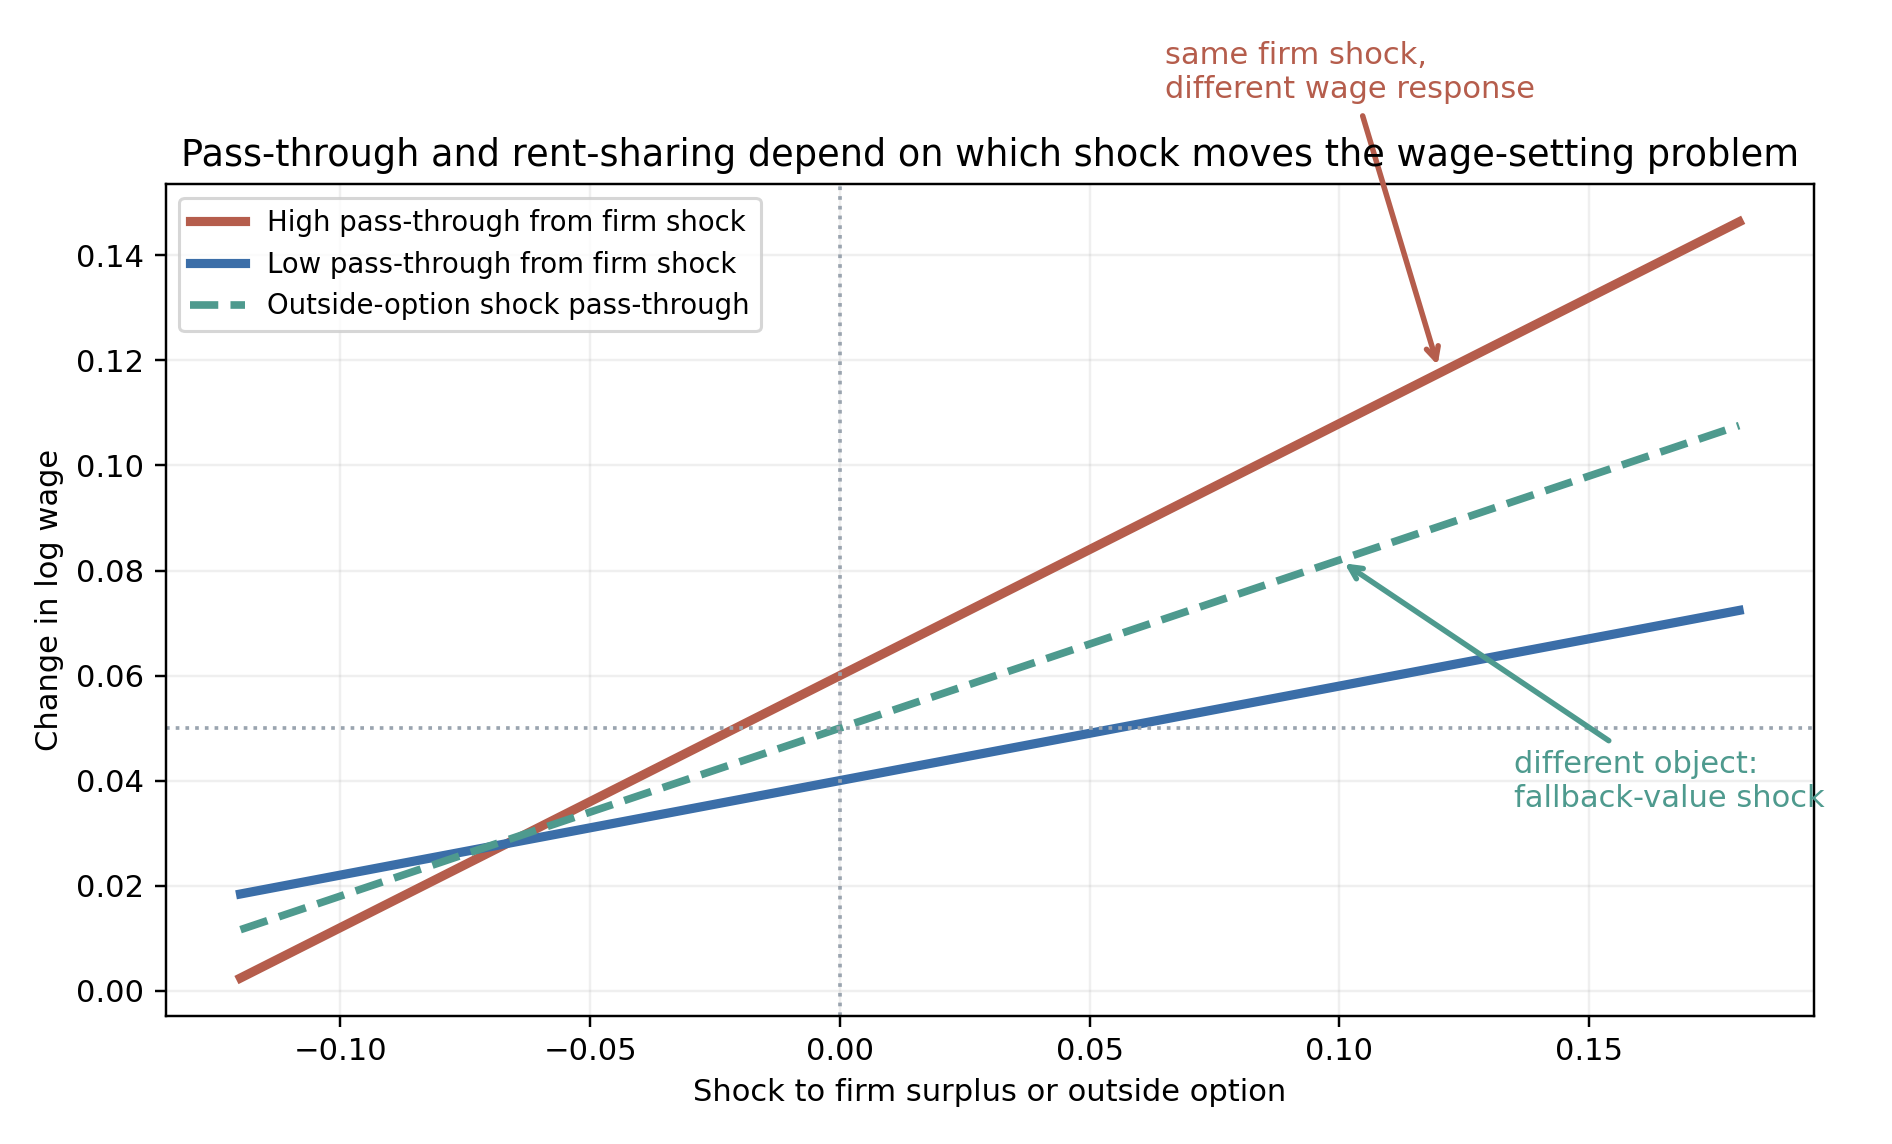
\includegraphics[height=0.7\textheight]{05-rent-sharing-pass-through.png}
\end{center}
\end{frame}

\begin{frame}{Frontier extension block}
\begin{itemize}
    \item Bargaining and within-firm inequality.
    \item Worker beliefs about outside options and firm-specific pay.
    \item Pay transparency, salary-history bans, and offer disclosure.
    \item Algorithmic pay-setting and remote hiring.
    \item Collective wage-setting as an alternative protocol rather than a later afterthought.
\end{itemize}
\end{frame}

\begin{frame}{Bridge to Week 6 monopsony}
\begin{itemize}
    \item Week 5 asks how wages are set once workers and firms meet.
    \item Week 6 asks how much wage-setting power firms have when labor supply to the firm is elastic but not infinite.
    \item Posting and bargaining are protocols; monopsony is the conduct environment in which those protocols operate.
\end{itemize}
\end{frame}

\begin{frame}{Takeaways}
\begin{itemize}
    \item Search models need an explicit wage-setting protocol.
    \item Posted wages, bargaining, and standardized or discretionary pay rules generate different empirical signatures.
    \item Reservation wages, outside offers, fallback values, and threat points must be kept separate.
    \item Rent-sharing evidence is informative, but it is not the whole structural wage-setting model.
\end{itemize}
\end{frame}

\appendix

\begin{frame}{Appendix: optional lab bridge}
\begin{itemize}
    \item Reproduce: dual-jobholder test in the spirit of Lachowska, Mas, Saggio, and Woodbury.
    \item Diagnose: is the paper testing posting, bargaining, or a wage-rule change?
    \item Transfer: public salary schedules or synthetic offer-and-separation panels.
    \item Extension: compare standardized and discretionary pay in teacher labor markets.
\end{itemize}
\end{frame}

\end{document}
